\section{Pasos para la instalación de TIBCO EBX}
\begin{quote}
  \textbf{Nota:} las rutas de este documento pueden variar según la configuración de cada equipo. 
\end{quote}

\begin{enumerate}

\item Descargar e instalar el kit de desarrollo de desarrollo \textbf{jdk-11.0.16\_windows-x64\_bin.zip.} Una vez instalado este kit de desarrollo, se debe colocar la variable de ambiente JAVA\_HOME con el valor \texttt{\textbf{C:\textbackslash ProgramFiles\textbackslash Java\textbackslash jdk-21.} } 

\item Crear una carpeta en la unidad de almacenamiento C:\ llamada EBX. 

\item Dentro de la carpeta C:\textbackslash EBX, crear las carpetas \textbf{EBXHome} y \textbf{TomCat}. 

\item Dentro de la carpeta \textbf{EBXHome}, se debe colocar el archivo \textbf{ebx.properties} el cual se encuentra dentro de la carpeta de instalación en la ruta \textbf{EBX\textbackslash 6.1.4\textbackslash ebx.software\textbackslash files}. 

\item Se debe descomprimir el servidor de aplicaciones \textbf{apache-tomcat.9.0.108-windows-x64}, después se accede al archivo descomprimido y se copia y pega la carpeta apache-tomcat.9.0.108 en la carpeta \textbf{C:\textbackslash EBX\textbackslash TomCat}. 
\begin{figure}[H]
    \centering
    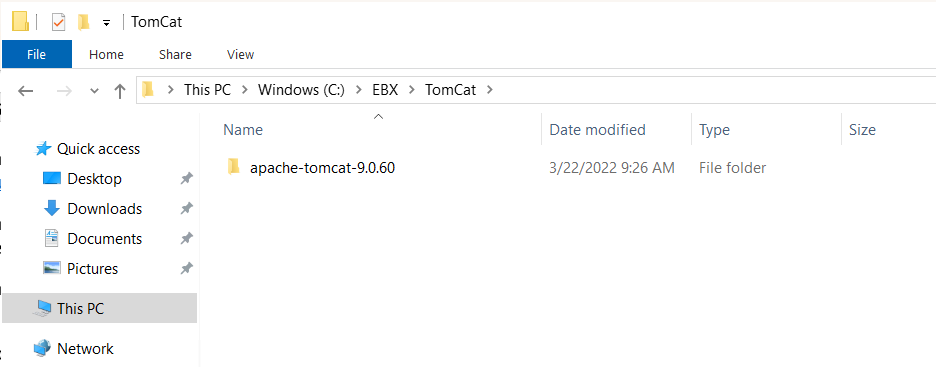
\includegraphics[width=0.7\textwidth]{Requerimientos/Instalacion/I09.png}
    \caption{Ubicación servidor Tomcat.}
\end{figure}

\item Se deberá editar el archivo \textbf{ebx.properties} que se encuentra dentro de la carpeta \textbf{C:\textbackslash EBX\textbackslash EBXHome;} en el cual se van a comentar las líneas que hacen referencia a una conexión de base de datos H2, como se muestra en la siguiente imagen (para comentar las líneas se deberá agregar el símbolo # antes del texto). 
\begin{figure}[H]
    \centering
    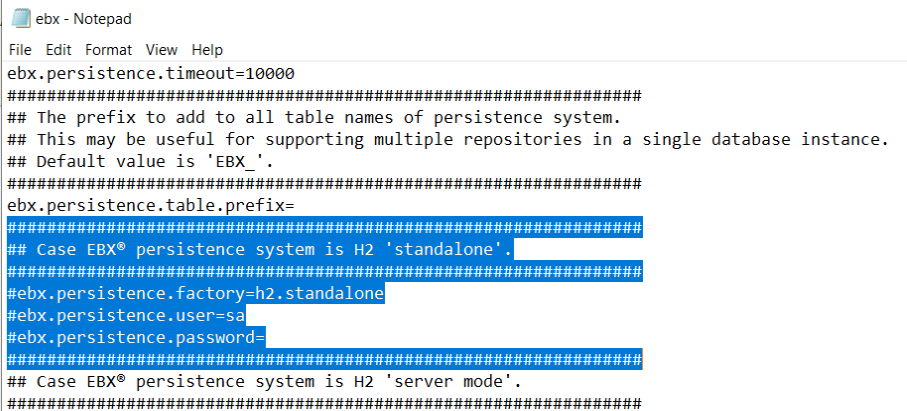
\includegraphics[width=0.7\textwidth]{Requerimientos/Instalacion/I10.png}
    \caption{Conexión a H2 comentada en ebx.properties}
\end{figure}

\item Posteriormente se procede a des comentar las líneas de código relativas a una conexión a base de datos Microsoft Azure SQL Server añadiendo los datos necesarios para realizar la conexión a la base de datos, tales como URL referencia, usuario y contraseña.  
\begin{figure}[H]
    \centering
    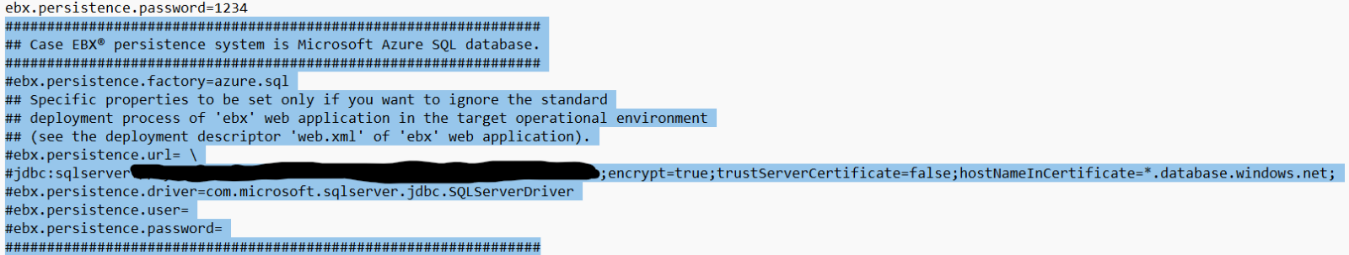
\includegraphics[width=0.7\textwidth]{Requerimientos/Instalacion/I11.png}
    \caption{Conexión a SQL Server.}
\end{figure}


\begin{quote}
  \textbf{Nota:} para cada servidor se deberá ejecutar el paso anterior, ya que son distintos servidores. 
\end{quote}

\item Editar el archivo catalina.properties que se encuentra en la ruta C:\textbackslash EBX\textbackslash TomCat\textbackslash apache.tomcat 9.0.108\conf agregando hasta el final del archivo las siguientes líneas de texto: 
\begin{figure}[H]
    \centering
    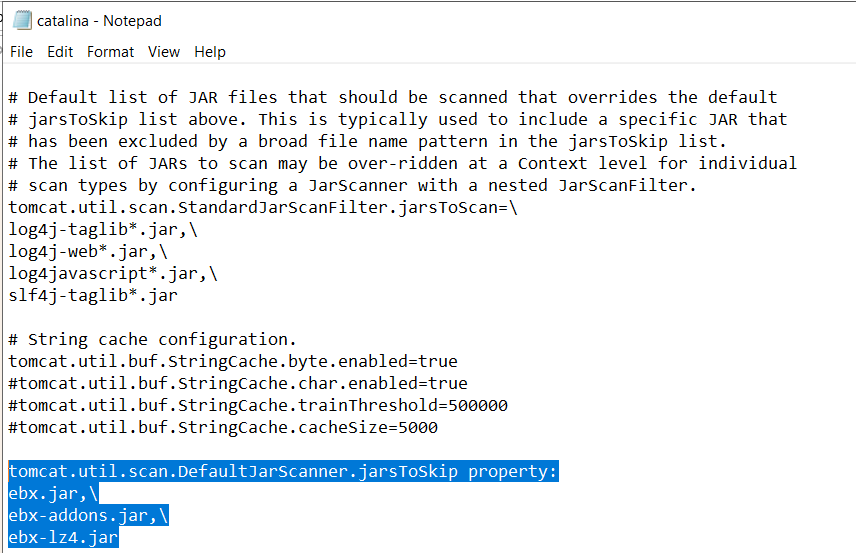
\includegraphics[width=0.7\textwidth]{Requerimientos/Instalacion/I12.png}
    \caption{Modificación archivo catalina.properties del servidor TomCat}
\end{figure}

\item Siguiendo la misma ruta del paso anterior, se editará el archivo server.xml donde se deberá identificar las siguientes líneas: 
\begin{figure}[H]
    \centering
    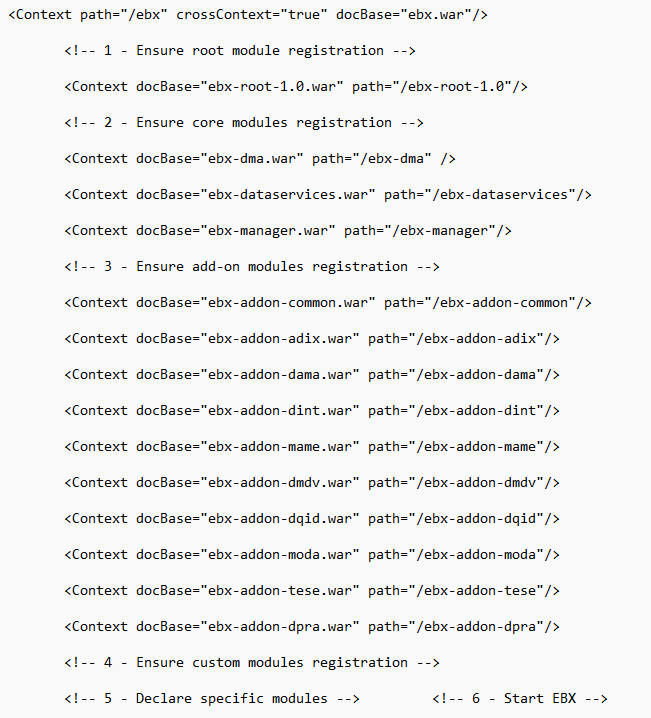
\includegraphics[width=0.7\textwidth]{Requerimientos/Instalacion/I13.png}
    \caption{Ubicación etiqueta Host dentro del archivo server.xml del servidor TomCat.}
\end{figure}

\item Para posteriormente agregar el siguiente código: 
\begin{figure}[H]
    \centering
    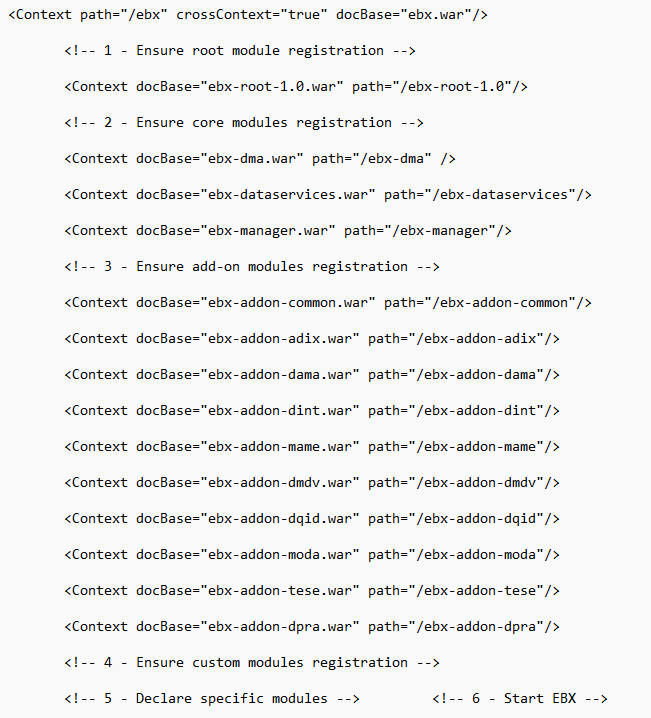
\includegraphics[width=0.7\textwidth]{Requerimientos/Instalacion/I14.png}
    \caption{Registro de instrucciones sobre módulos y acciones del servidor.}
\end{figure}

\item Ingresar a la ruta del instalador EBX\textbackslash Add-ons\textbackslash 6.1.4\textbackslash wars, en donde se deben copiar todos los archivos con extensión .war. Después esos archivos copiados se deben pegar en la ruta C:\textbackslash EBX\textbackslash TomCat\textbackslash apache-tomcat-9.0.108\textbackslash webapps. 

\item Se usará third party con extensión .jar, los cuales son mssql-jdbc-8.4.1.jre8.jar, org.json.jar y mail.jar. Estos archivos deberán de estar alojados en: C:\textbackslash EBX\textbackslash TomCat\textbackslash apache-tomcat 9.0.108\textbackslash lib. 

\item Se debe ingresar a la ruta EBX Add-ons\textbackslash 6.1.4\textbackslash lib y copiar los únicos dos archivos presentes y pegarlos en C:\textbackslash EBX\textbackslash TomCat\textbackslash apache-tomcat 9.0.108\textbackslash lib. 

\item Ingresar a la carpeta del instalador en la ruta EBX Add-ons\textbackslash 5.1.1\textbackslash EBX5-addons\textbackslash EBX5-addons\textbackslash wars, copiar todos los archivos .war y pegarlos en la ruta C:\textbackslash EBX\textbackslash TomCat\textbackslash apache-tomcat-9.0.108\textbackslash webapps. 

\item Ingresar a la ruta del instalador: TIBCO\textbackslash EBX\textbackslash 6.1.4\textbackslash TIB\_ebx\_6.1.4\textbackslash ebx.software\textbackslash lib, realizar la copia del archivo ebx.jar y pegarlo en la ruta donde se encuentran los archivos de inicialización para la aplicación de EBX: C:\textbackslash EBX\textbackslash TomCat\textbackslash apache-tomcat 9.0.108\textbackslash lib. 

\item Se deberá ingresar a la ruta C:\textbackslash EBX\textbackslash TomCat\textbackslash apache-tomcat-9.0.108\textbackslash bin para editar el archivo startup.bat; en el cual se debe ubicar el cursor en la antepenúltima línea del documento e insertar el siguiente texto: 
\begin{figure}[H]
    \centering
    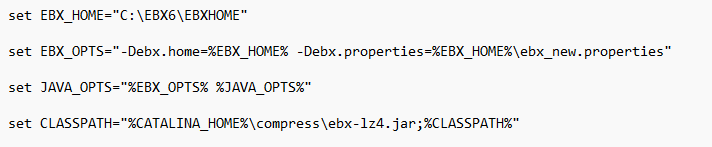
\includegraphics[width=0.7\textwidth]{Requerimientos/Instalacion/I15.png}
    \caption{Declaración de variables de entorno dentro de archivo startup.bat.}
\end{figure}

\item Colocar la variable de ambiente CATALINA\_HOME con el valor: C:\textbackslash EBX\textbackslash TomCat\textbackslash apache-tomcat-9.0.108. 

\item Abrir una terminal nueva de Windows, dirigirse a la siguiente ruta C:\textbackslash EBX\textbackslash TomCat\textbackslash apache-tomcat-9.0.108\textbackslash bin para después ejecutar el comando startup.bat y esperar 10 minutos. 

\item Después de los 10 minutos de espera, se dirige a un navegador, por ejemplo, Mozilla o Chrome, e ingresar a la siguiente dirección: ip-server:8080\textbackslash ebx. 
\end{enumerate}

%% inicio de sub sección

\subsection{Instalación del repositorio de TIBCO EBX }

\begin{enumerate}
    \item Una vez instalado de forma correcta EBX, se procede a abrir una línea de comando ingresando a la carpeta apache tomcat mediante el comando cd \textbackslash \%CATALINA\_HOME\%. Posteriormente se ingresa a la carpeta bin mediante el comando cd bin e inicia el archivo startup.bat. 
\begin{figure}[H]
    \centering
    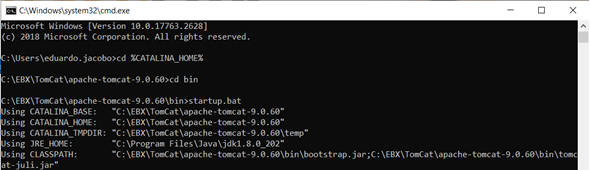
\includegraphics[width=0.7\textwidth]{Requerimientos/Instalacion/I16.png}
    \caption{Iniciando archivo startup.bat.}
\end{figure}

\item Una vez inicializado el archivo startup.bat, se abrirá una ventana Tomcat la cual informará del estado del servidor. Habrá que esperar a que se indique que el servidor está listo como muestra la siguiente imagen. 
\begin{figure}[H]
    \centering
    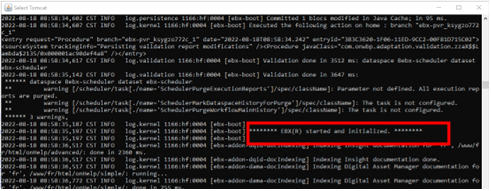
\includegraphics[width=0.7\textwidth]{Requerimientos/Instalacion/I17.png}
    \caption{Estado del servidor durante su ejecución.}
\end{figure}

\item Una vez iniciado el servidor, entrar al navegador web con el siguiente enlace http://localhost:8080/ebx para iniciar el instalador de repositorios de TIBCO EBX. 

\item Una vez iniciada la instalación del repositorio, se solicitará ingresar el IP del repositorio; para esto dar clic en el botón “GENERATE” que se encuentra a la derecha del text box Repository ID. Esto generará automáticamente un ID de repositorio. Después se debe colocar el nombre del repositorio en el text box Repository Label. 

\begin{figure}[H]
    \centering
    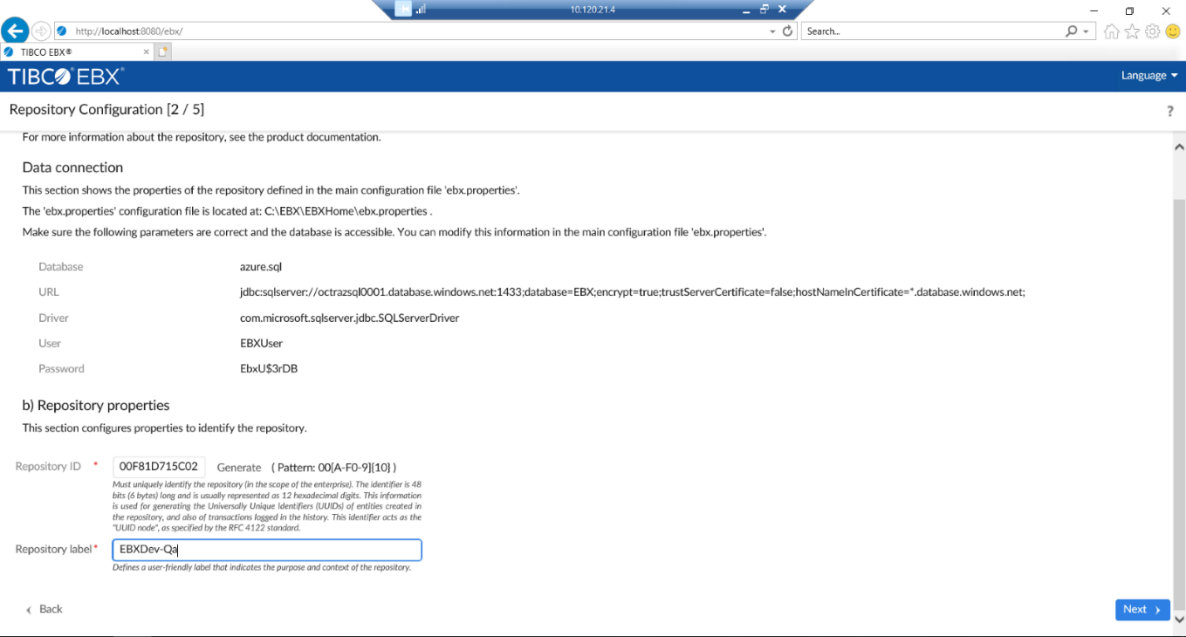
\includegraphics[width=0.7\textwidth]{Requerimientos/Instalacion/I18.png}
    \caption{Configuración sobre datos del repositorio.}
\end{figure}

\item Después de colocar los datos del repositorio, se solicitará la creación de un usuario base con el nombre del usuario y la contraseña deseada y se repite dicha contraseña como confirmación. 

\begin{figure}[H]
    \centering
    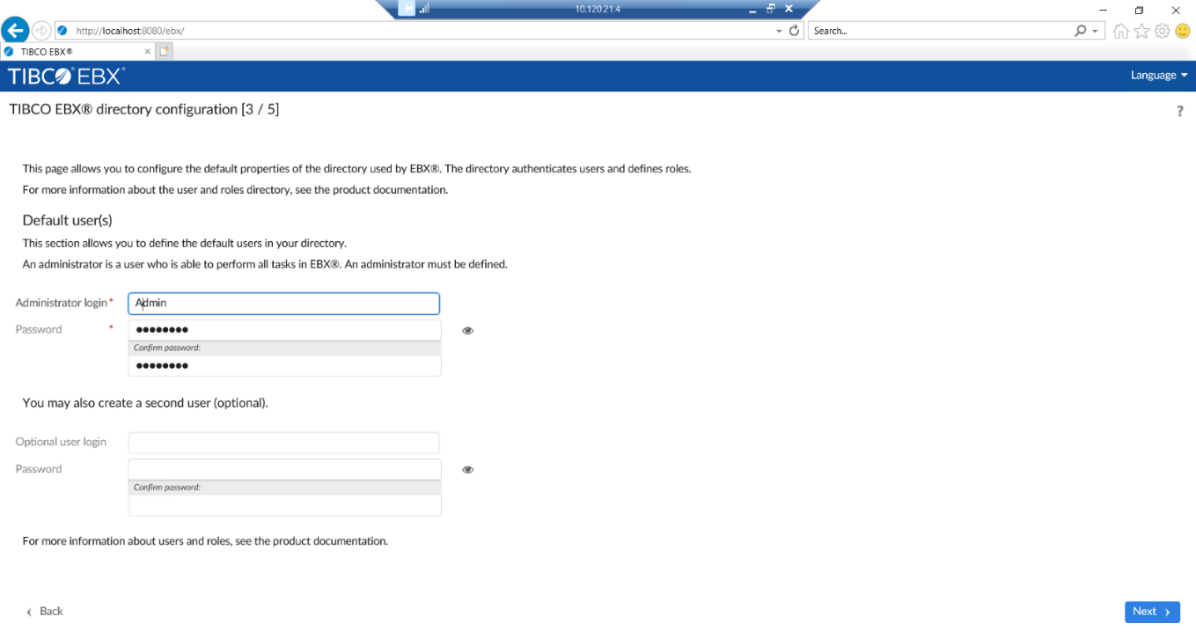
\includegraphics[width=0.7\textwidth]{Requerimientos/Instalacion/I19.png}
    \caption{Creación del usuario base del repositorio.}
\end{figure}

\item Posteriormente, la pantalla mostrará un resumen de la información ingresada a EBX (datos de la conexión, propiedades del repositorio y usuario).

\begin{figure}[H]
    \centering
    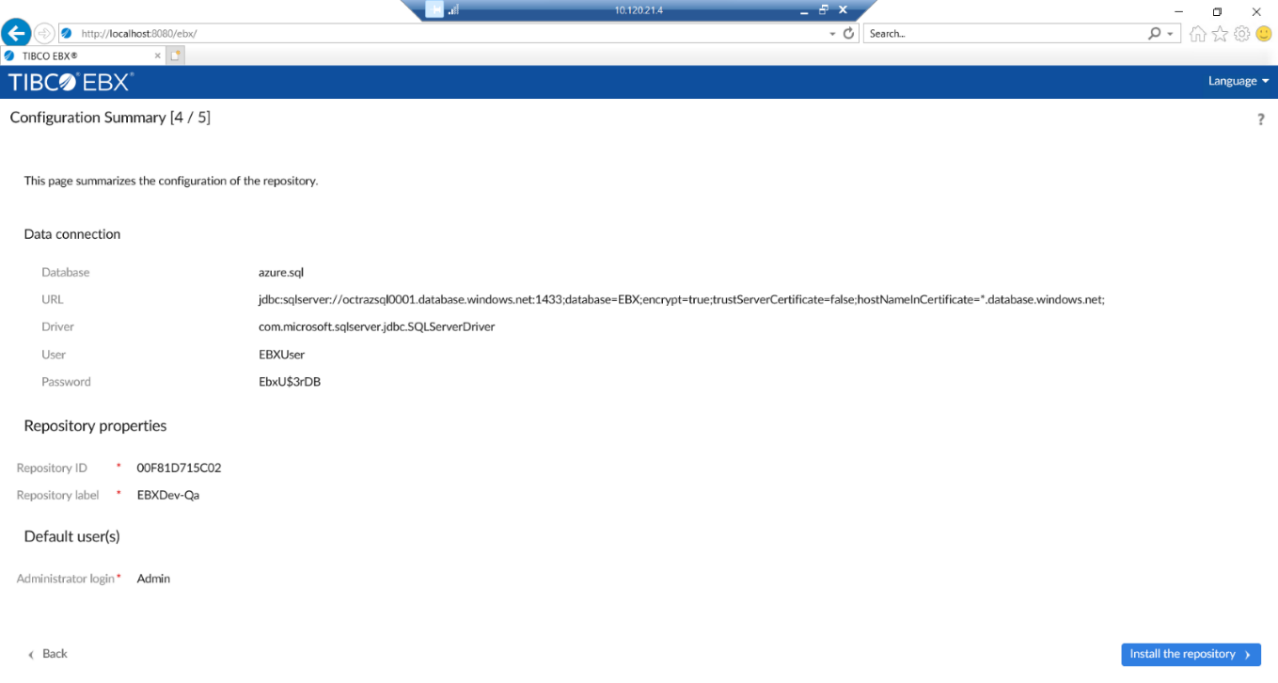
\includegraphics[width=0.7\textwidth]{Requerimientos/Instalacion/I20.png}
    \caption{Resumen de información ingresada sobre repositorio y usuario base.}
\end{figure}

\item Ya instalado el repositorio, se habilita el log in y se podrá ingresar los datos de usuario para poder hacer uso de TIBCO EBX. 

\begin{figure}[H]
    \centering
    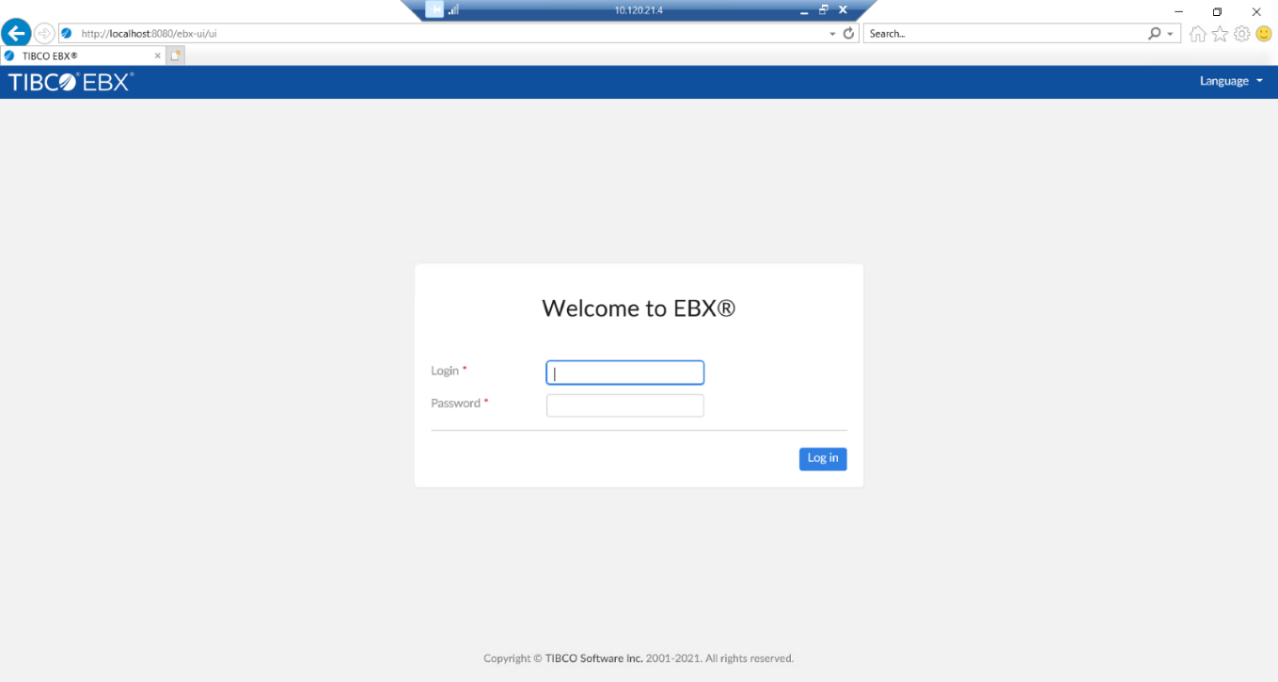
\includegraphics[width=0.7\textwidth]{Requerimientos/Instalacion/I21.png}
    \caption{Login de la herramienta TIBCO EBX.}
\end{figure}

\item Para cerrar el servidor una vez terminado su uso, se debe regresar a la línea de comando e iniciar el archivo shutdown.bat. 

\begin{figure}[H]
    \centering
    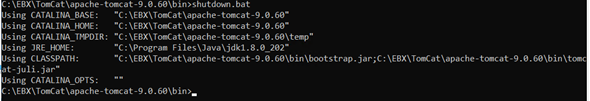
\includegraphics[width=0.7\textwidth]{Requerimientos/Instalacion/I22.png}
    \caption{Apagado del servidor.}
\end{figure}

\end{enumerate}


\subsubsection{Encendido}

Para iniciar el servidor y empezar su uso, se debe ingresar a la línea de comando ingresando a la carpeta apache tomcat mediante el comando \textbf{cd \%CATALINA\_HOME\%}, yendo a la carpeta bin e iniciar el archivo startup.bat. 

\begin{figure}[H]
    \centering
    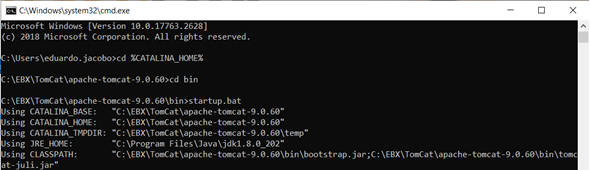
\includegraphics[width=0.7\textwidth]{Requerimientos/Instalacion/I25.png}
    \caption{Encendido del servidor.}
\end{figure}


\subsubsection{Apagado }

Para cerrar el servidor una vez terminado su uso, se debe regresar a la línea de comando e iniciar el archivo shutdown.bat. 

\begin{figure}[H]
    \centering
    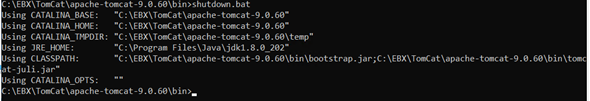
\includegraphics[width=0.7\textwidth]{Requerimientos/Instalacion/I26.png}
    \caption{Apagado del servidor.}
\end{figure}

\subsection{Configuración del certificado}

\begin{enumerate}
    \item Dentro la carpeta conf, colocar el archivo .pfx perteneciente al certificado de seguridad.

\begin{figure}[H]
    \centering
    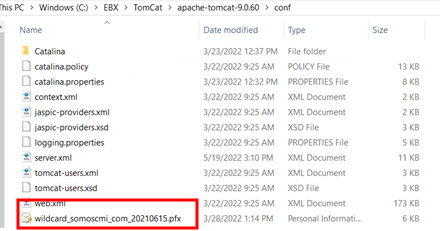
\includegraphics[width=0.7\textwidth]{Requerimientos/Instalacion/I27.png}
    \caption{Ubicación para el archivo .pfx.}
\end{figure}

Al tener el archivo en la carpeta específica, instalar el certificado correspondiente. 

\begin{figure}[H]
    \centering
    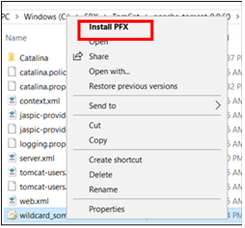
\includegraphics[width=0.5\textwidth]{Requerimientos/Instalacion/I28.png}
    \caption{Instalación del certificado de seguridad.}
\end{figure}

\item Cuando se selecciona Install PFX, se desplegará la ventana de instalación como se muestra a continuación. Donde se debe seleccionar Current User y después Next. 

\begin{figure}[H]
    \centering
    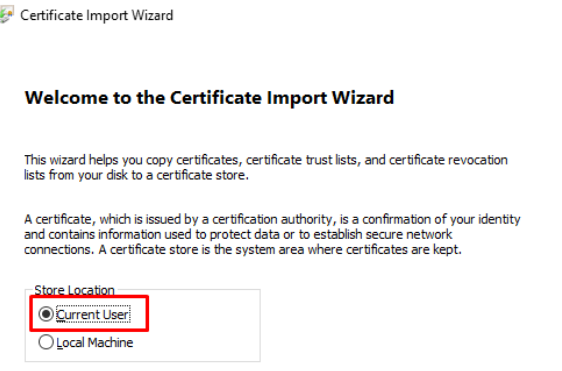
\includegraphics[width=0.7\textwidth]{Requerimientos/Instalacion/I29.png}
    \caption{Ventana inicial del instalador.}
\end{figure}

\item Al presionar Next, se abrirá una ventana donde por defecto se selecciona el archivo a instalar. Si éste no es el caso, se debe de seleccionar el archivo tipo .pfx y presionar Next. 

\begin{figure}[H]
    \centering
    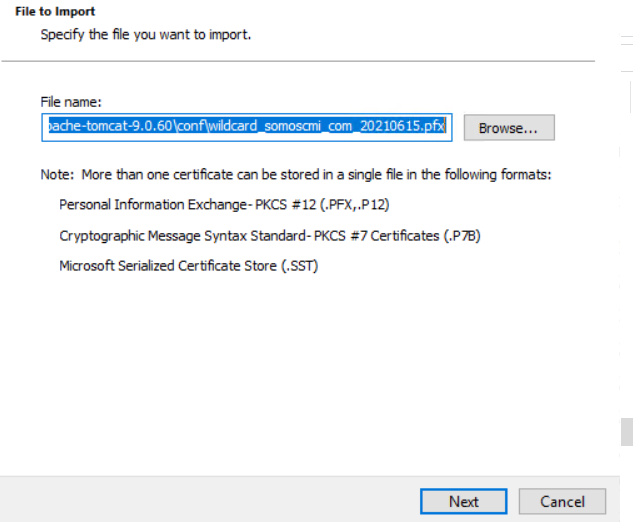
\includegraphics[width=0.7\textwidth]{Requerimientos/Instalacion/I30.png}
    \caption{Ubicación del archivo .pfx dentro del instalador.}
\end{figure}

\item Dentro de los pasos de instalación, es necesario un paso de seguridad; por lo cual se despliega una ventana en la cual se solicita ingresar la contraseña del certificado en cuestión. Además, como paso adicional, se deben marcar las casillas que se muestran en la imagen. 

\begin{figure}[H]
    \centering
    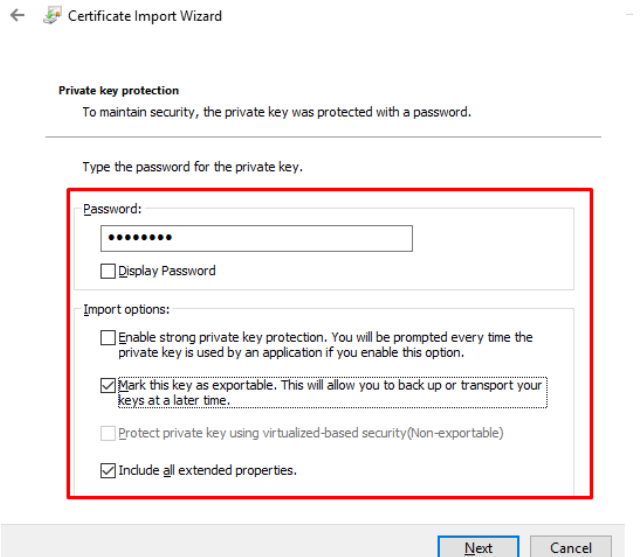
\includegraphics[width=0.5\textwidth]{Requerimientos/Instalacion/I31.png}
    \caption{Paso de seguridad - Ingreso de credenciales del certificado.}
\end{figure}

\item El siguiente paso consta de seleccionar la casilla marcada, y dar Next. 

\begin{figure}[H]
    \centering
    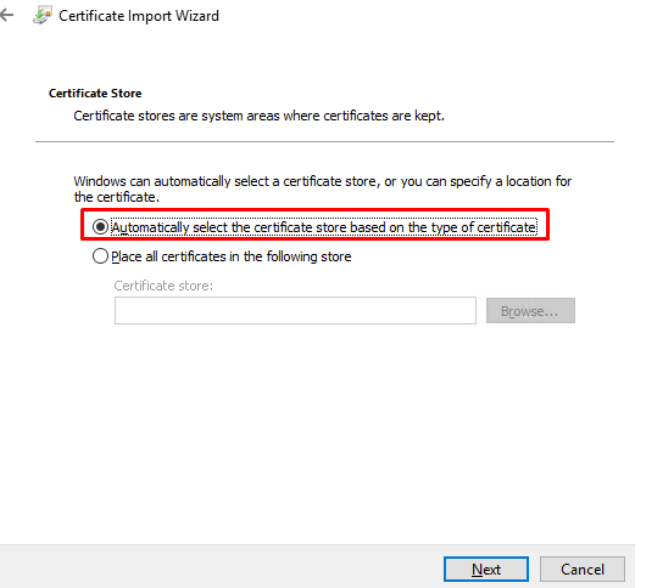
\includegraphics[width=0.5\textwidth]{Requerimientos/Instalacion/I32.png}
    \caption{Selección del Cerificate Store.}
\end{figure}

\item Para finalizar la instalación, se verifica la información ingresada y presiona Finish. 

\begin{figure}[H]
    \centering
    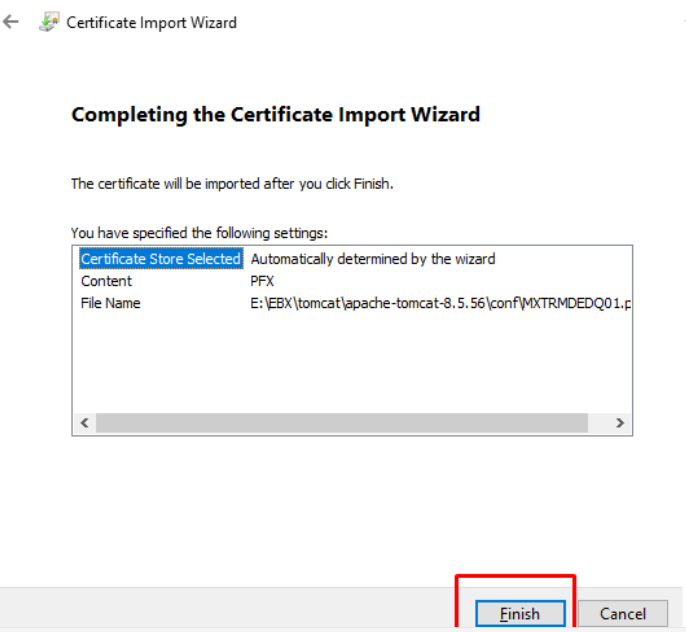
\includegraphics[width=0.5\textwidth]{Requerimientos/Instalacion/I33.png}
    \caption{Validación de información sobre el certificado.}
\end{figure}

\item Con los pasos anteriores se termina la instalación del certificado de seguridad dentro el servidor; los siguientes pasos son para el uso del certificado recién instalado en la aplicación de EBX. 

Dentro la misma ruta donde se colocó el archivo .pfx, se encuentra el archivo server.xml, el cual se debe de abrir para su edición. 

Se debe de editar la etiqueta Connector agregando keystoreFile, a este atributo se le dará el valor de la dirección donde se encuentra el archivo .pfx recién instalado como se muestra en la siguiente imagen. Además de agregar el atributo keystorePass; el valor dado será la contraseña del certificado de seguridad. 

\begin{figure}[H]
    \centering
    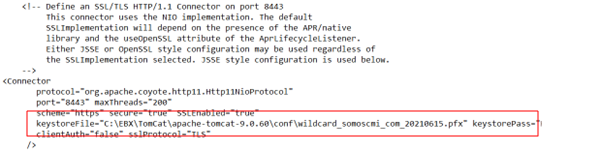
\includegraphics[width=0.7\textwidth]{Requerimientos/Instalacion/I34.png}
    \caption{Edición del archivo server.xml con los datos del certificado.}
\end{figure}

\item Con esta configuración se puede iniciar el servicio y comprobar su correcta instalación. Para esto hay dos formas de comprobarlo.  

\begin{itemize}
    \item La primera es estar dentro del servidor y esperar a que el servicio termine de iniciar, dentro de un navegador ingresar al servicio de TIBCO EBX con la URL https://localhost:8443/ebx donde se desplegará el login perteneciente a TIBCO EBX. 
    
    \item La segunda forma es dentro los logs del servicio de Tomcat, donde se puede ver que el servicio de https se ha iniciado. 

\end{itemize}

\begin{figure}[H]
    \centering
    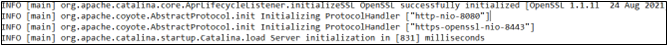
\includegraphics[width=0.7\textwidth]{Requerimientos/Instalacion/I35.png}
    \caption{Comprobación del log del servicio.}
\end{figure}

\end{enumerate}

%% -------- PRUEBAS DE INSTALACION -----------

\section{Pruebas de funcionamiento}

\begin{enumerate}
    \item Creación de modelo de datos. 

    \begin{figure}[H]
        \centering
        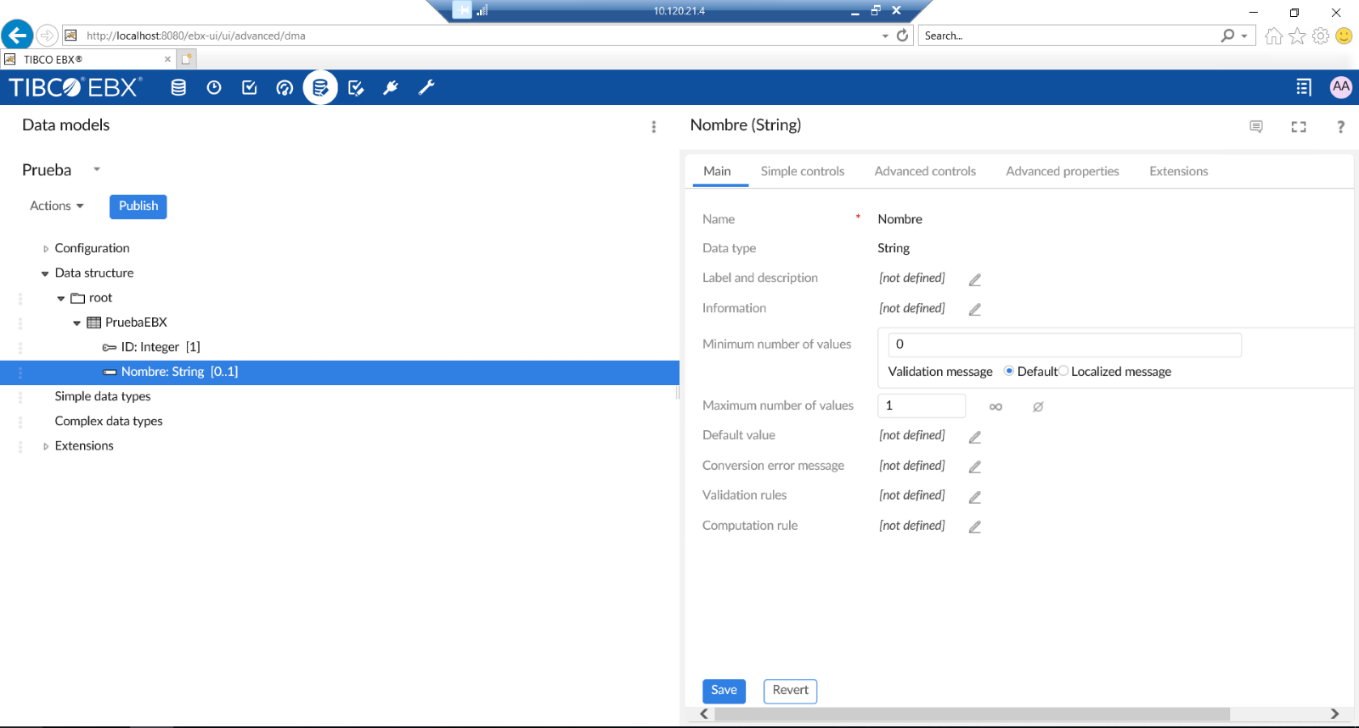
\includegraphics[width=0.7\textwidth]{Requerimientos/PruebasInstalacion/PF01.png}
        \caption{Modelo de datos básico en TIBCO EBX.}
    \end{figure}
    
    \item Creación de dataspace. 

    \begin{figure}[H]
        \centering
        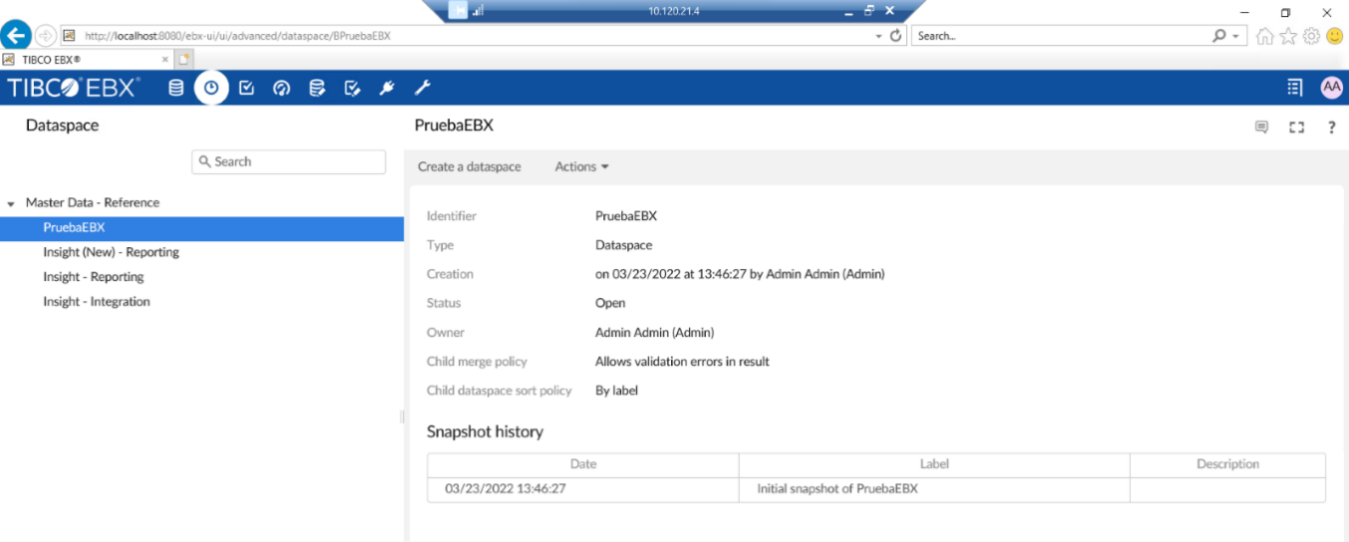
\includegraphics[width=0.7\textwidth]{Requerimientos/PruebasInstalacion/PF02.png}
        \caption{Espacio de datos en TIBCO EBX.}
    \end{figure}

    \item Publicación del dataset.
     \begin{figure}[H]
        \centering
        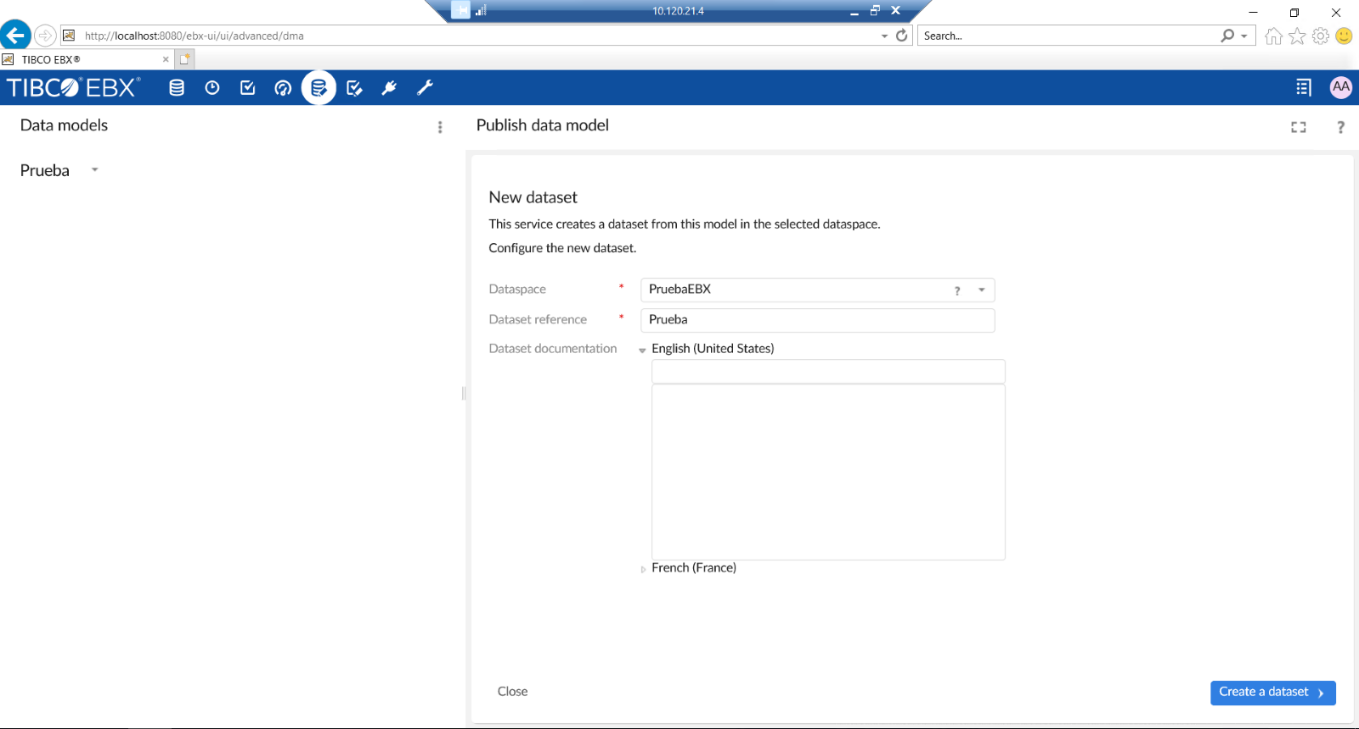
\includegraphics[width=0.7\textwidth]{Requerimientos/PruebasInstalacion/PF03.png}
        \caption{Publicación del modelo en el conjunto de datos.}
    \end{figure}
    
    \item Fin de la publicación de modelo de datos en conjunto de datos (DATASET). 
    \begin{figure}[H]
        \centering
        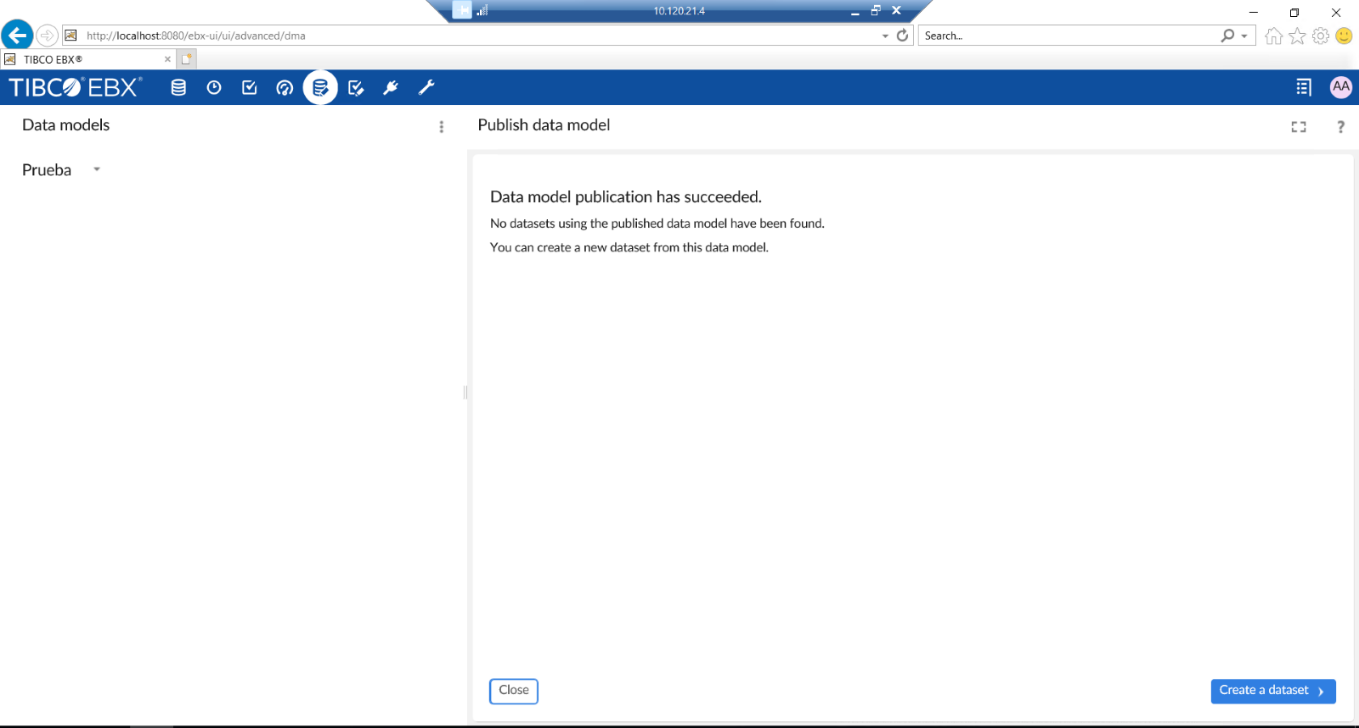
\includegraphics[width=0.7\textwidth]{Requerimientos/PruebasInstalacion/PF04.png}
        \caption{Fin de la publicación del modelo de datos}
    \end{figure}
    
    \item Publicación del dataset exitosa e ingreso exitoso de datos de prueba. 
    \begin{figure}[H]
        \centering
        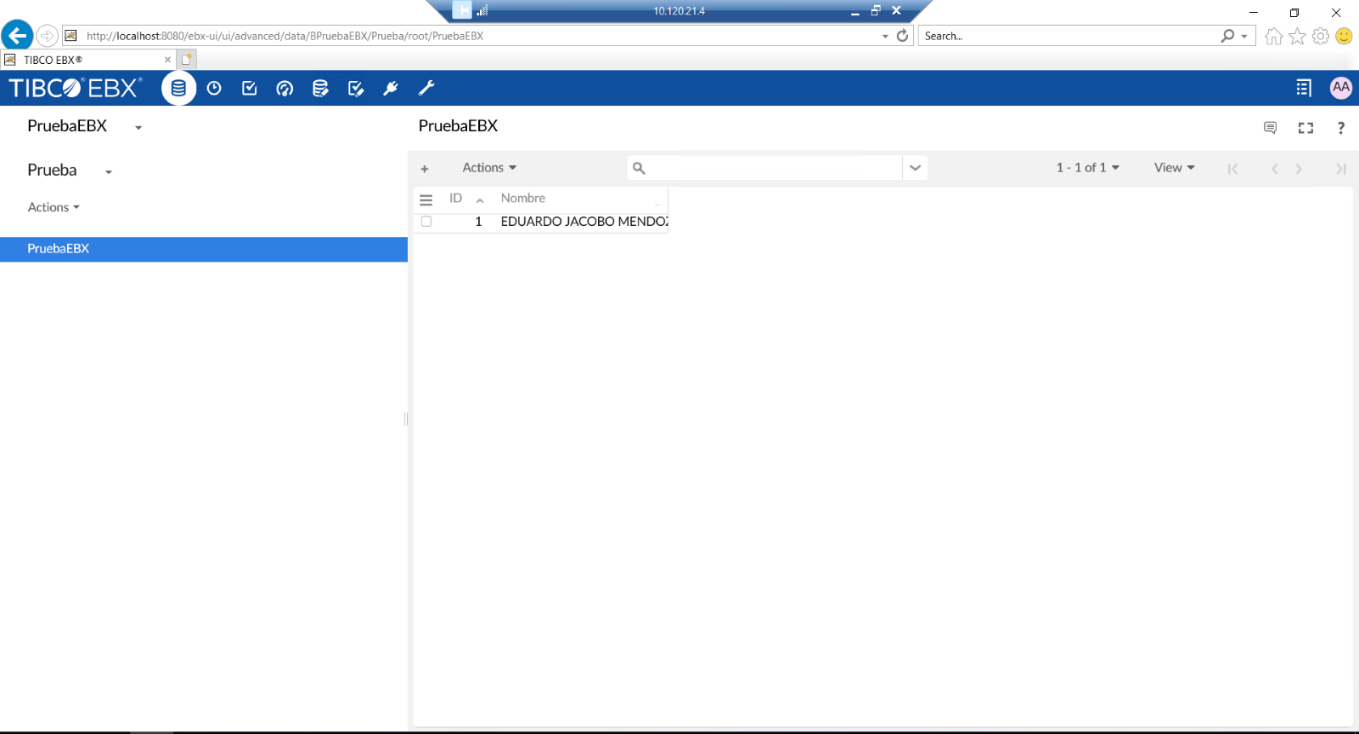
\includegraphics[width=0.7\textwidth]{Requerimientos/PruebasInstalacion/PF05.png}
        \caption{Prueba de ingreso de datos dentro del conjunto de datos}
    \end{figure}
\end{enumerate}